\subsection{Desarrollo embrionario}\label{sec:exp2_embriones}

\subsubsection{Datos de origen}

Se utiliza un conjunto de datos público de imágenes \textit{time-lapse} de embriones humanos en incubadora (Gomez et al., 2022), en el plano focal central. Contiene 704 embriones con una mediana de 548 imágenes cada uno (mínimo 137, máximo 1140), en escala de grises de $500 \times 500$ píxeles, desde el cigoto hasta mórula o blastocisto.

Cada imagen muestra el pozo de cultivo, la \textit{zona pelúcida} (una capa que envuelve al embrión y se observa como un anillo gris con textura fina) y, dentro de ella, las células. El conjunto presenta tres particularidades que la limpieza debe resolver: 211 embriones repiten todas sus imágenes en una subcarpeta (se toma una sola copia), los números de imagen no tienen ceros a la izquierda (se ordenan numéricamente) y en algunas secuencias el embrión sale de cuadro al final.

\subsubsection{Limpieza}

\begin{enumerate}
	\item \textbf{Localización de la zona pelúcida.} El círculo se calcula una sola vez por embrión, para que el ruido de la detección no aparezca como un cambio de escala entre imágenes. En una imagen aislada el borde de la zona es demasiado tenue para la transformada de Hough, pero la zona permanece fija mientras las células se mueven: la desviación estándar temporal de cada píxel dibuja el interior de la zona como un disco nítido (figura \ref{fig:embryo_std}), al que se ajusta un círculo con RANSAC. El borde exterior se ubica donde termina la textura fina de la zona en la imagen media.
	\item \textbf{Imágenes inválidas.} Se descartan las imágenes sin textura dentro del círculo (embrión fuera de cuadro) y se conserva el tramo continuo más largo de imágenes válidas.
	\item \textbf{Recorte y reducción.} Se recorta el cuadrado del círculo exterior y se reduce a $n \times n$ por promedio de área, de modo que cada embrión queda normalizado al tamaño de su zona pelúcida.
	\item \textbf{Estados.} Se definen cinco estados (tabla \ref{tab:embryo_estados}). Los dos primeros se obtienen por geometría; dentro de la zona, los bordes celulares se detectan con el operador de Sobel sobre la imagen reducida, con un umbral de Otsu calculado con todas las imágenes del embrión.
	\item \textbf{Reducción de ruido.} Se aplica histéresis a los bordes (un borde débil se conserva solo si está conectado a uno fuerte) y una mediana temporal de tres imágenes. La apertura morfológica se descartó porque elimina las membranas, que miden una o dos celdas de grosor (figura \ref{fig:embryo_ruido}).
\end{enumerate}

\begin{figure}[H]
	\centering
	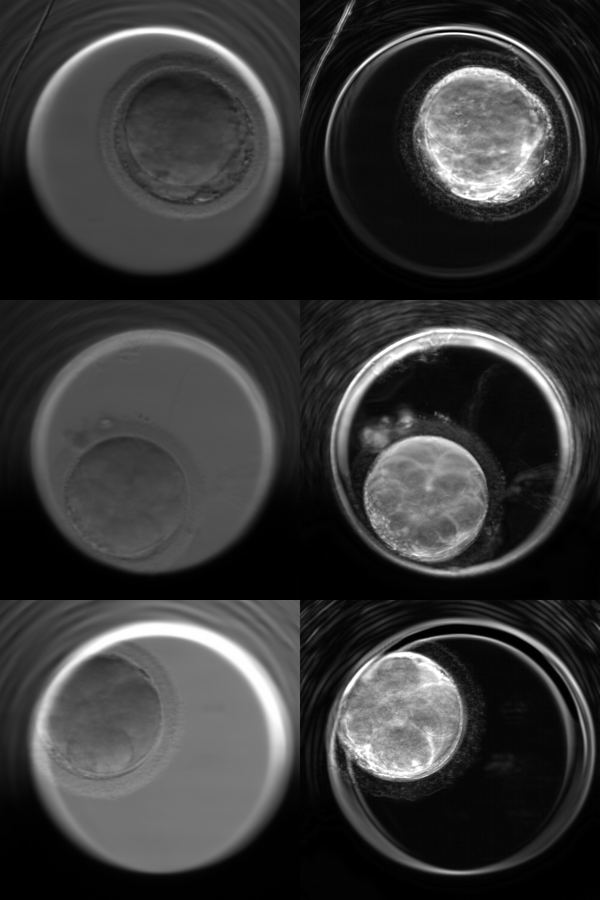
\includegraphics[width=0.6\linewidth]{img/embryo_std_temporal.png}
	\caption{Media temporal (izquierda) y desviación estándar temporal (derecha) de tres embriones. El interior de la zona pelúcida aparece como un disco de alta variación.}
	\label{fig:embryo_std}
\end{figure}

\begin{table}[H]
	\centering
	\begin{tabular}{c|l|p{0.55\linewidth}}
		\hline
		\textbf{Estado} & \textbf{Nombre} & \textbf{Regla} \\ \hline
		0 & Fuera & Fuera del círculo exterior de la zona pelúcida. \\ \hline
		1 & Zona pelúcida & Anillo entre el círculo interior y el exterior. \\ \hline
		2 & Interior & Interior de la zona que no es borde ni brillo. \\ \hline
		3 & Borde & Gradiente de Sobel sobre el umbral de Otsu, con histéresis y mediana temporal. \\ \hline
		4 & Brillo & Intensidad mayor a la media más 1.5 desviaciones estándar del interior, en celdas que no son borde. \\ \hline
	\end{tabular}
	\caption{Estados de la segmentación de embriones.}
	\label{tab:embryo_estados}
\end{table}

\begin{figure}[H]
	\centering
	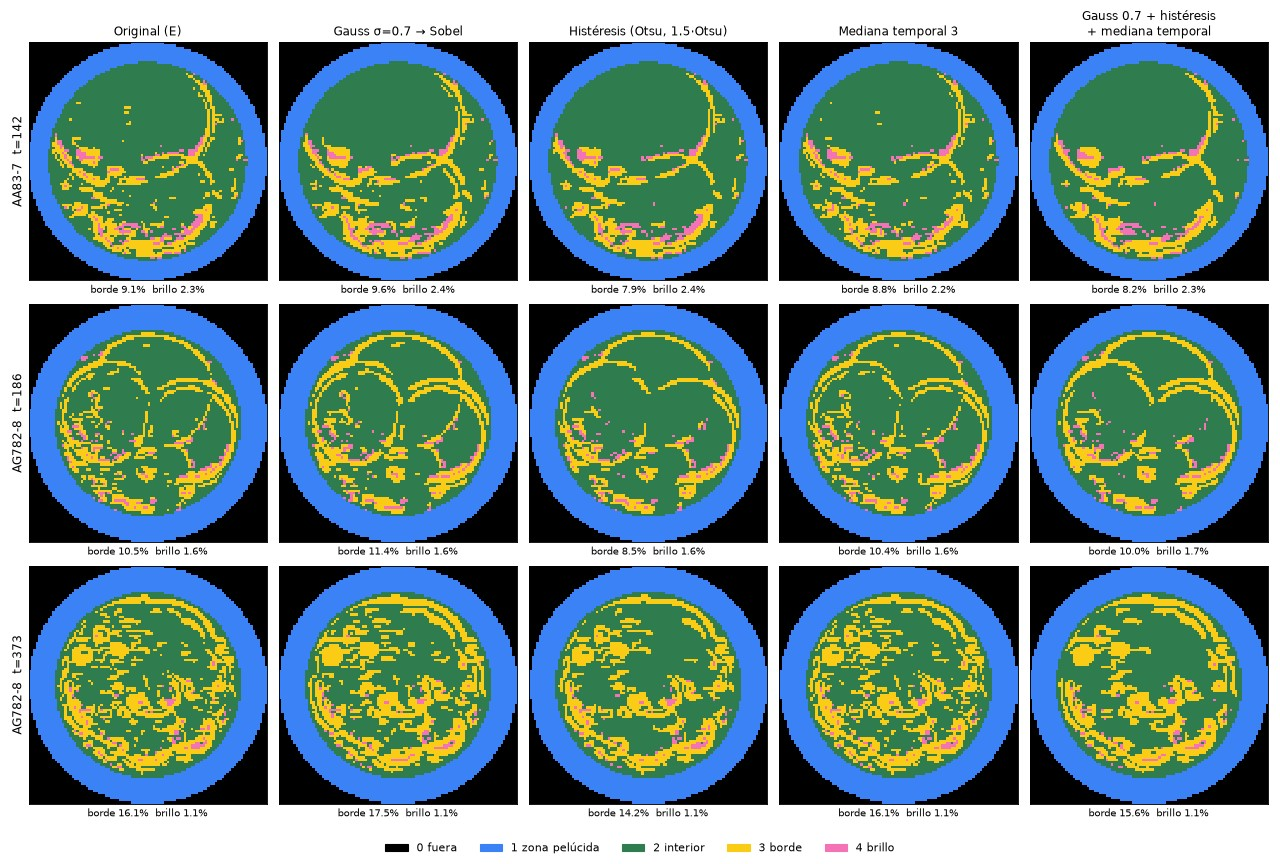
\includegraphics[width=\linewidth]{img/embryo_ruido.jpg}
	\caption{Alternativas de reducción de ruido sobre los bordes detectados.}
	\label{fig:embryo_ruido}
\end{figure}

La limpieza se aplicó a tres embriones. En el embrión AG782-8 se conservan 374 de 565 imágenes, desde el cigoto hasta mórula (figura \ref{fig:embryo_frames}); la fracción de borde dentro del embrión crece con el número de células, de 7.3\% al inicio a 25.5\% al final (figura \ref{fig:embryo_states}).

\begin{figure}[H]
	\centering
	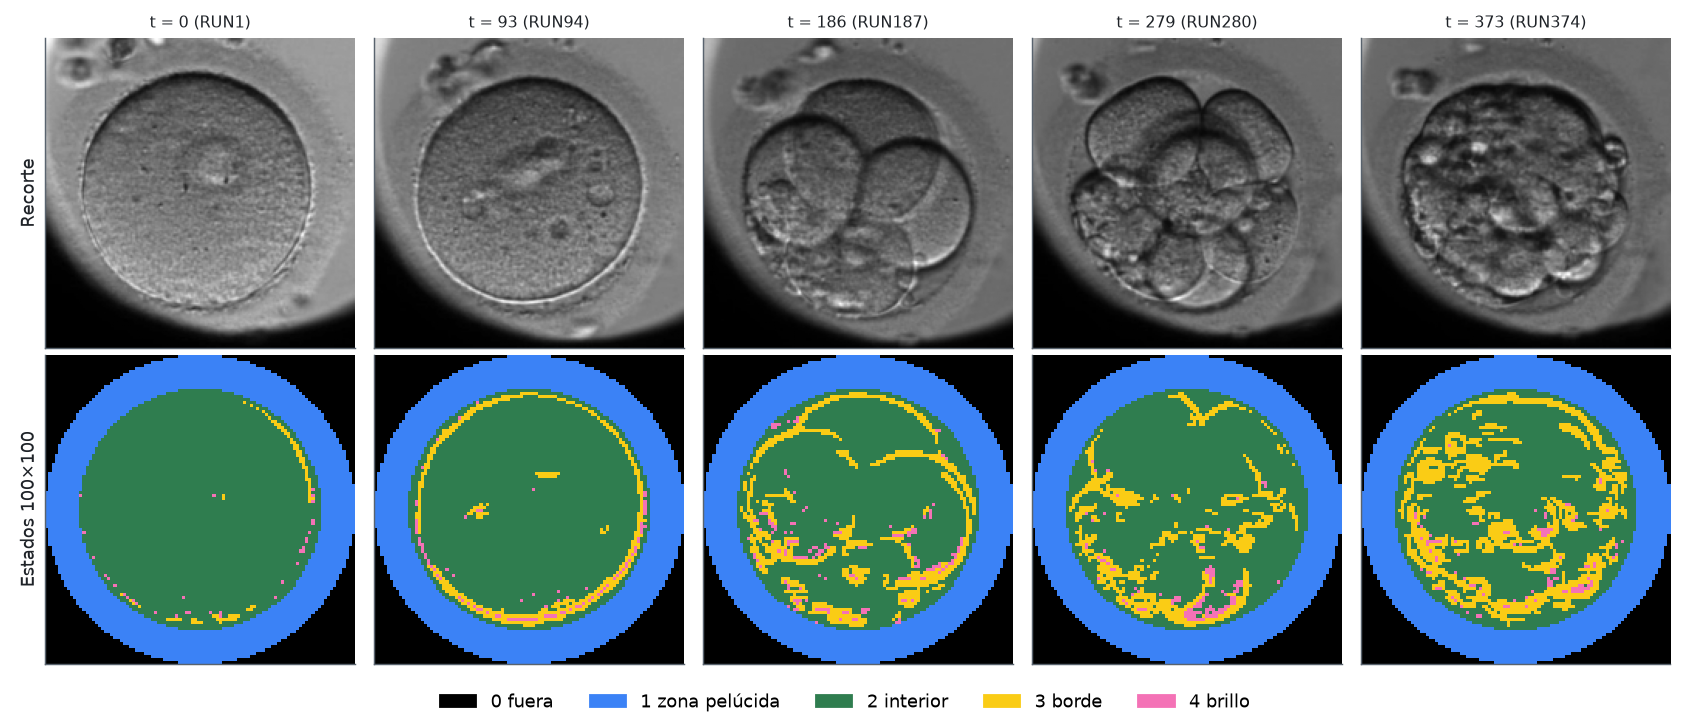
\includegraphics[width=\linewidth]{img/embryo_frames.png}
	\caption{Recorte y estados en cinco momentos del embrión AG782-8.}
	\label{fig:embryo_frames}
\end{figure}

\begin{figure}[H]
	\centering
	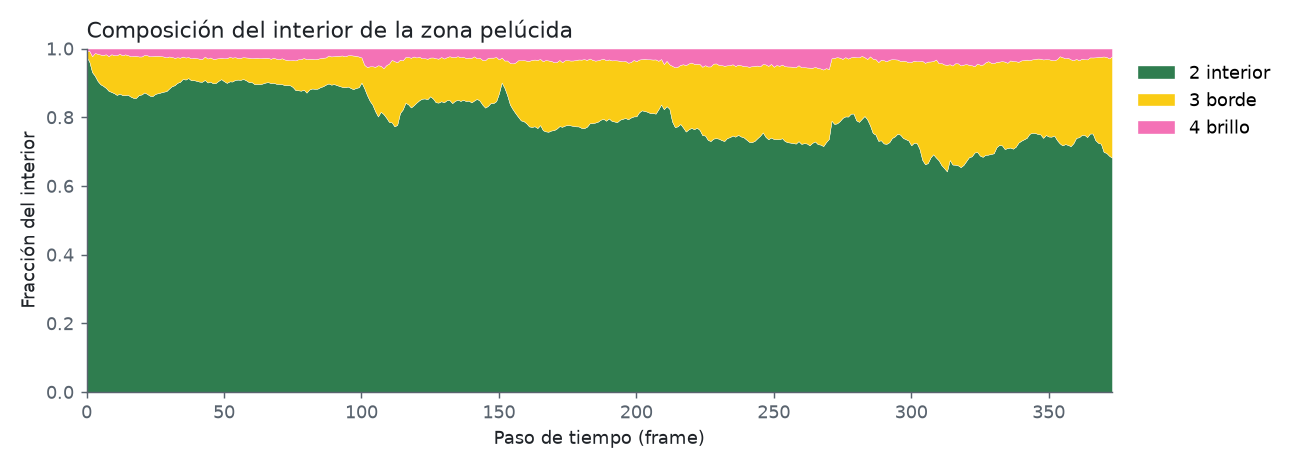
\includegraphics[width=0.9\linewidth]{img/embryo_states.png}
	\caption{Composición del interior de la zona pelúcida del embrión AG782-8 a lo largo del tiempo.}
	\label{fig:embryo_states}
\end{figure}

\subsubsection{Entrenamiento y resultados}

\TODO{Procesar los 704 embriones y descartar los que estén pegados a la pared del pozo, cuyo borde brillante aparece como una franja fija de estados 3 y 4.}

\TODO{Entrenar el autómata celular neuronal (5 estados, salida multiclase) y comparar la evolución generada contra la observada.}
